% status: 0
% chapter: REST

\title{Azure Virtual Machine deployment using Swagger REST Service}


\author{Ankita Alshi}
\affiliation{%
  \institution{Indiana University}
  \city{Bloomington} 
  \state{IN} 
  \postcode{47404}
  \country{USA}}
\email{aralshi@iu.edu}


% The default list of authors is too long for headers
\renewcommand{\shortauthors}{Ankita Alshi}

\begin{abstract}
This project demonstrates advantage of using Swagger codegen to create a REST
service using swagger specification yaml file. Project uses Azure python APIs
to connect and communicate with azure to provide easy way to create new
instance of resources like virtual machine or virtual network on. Clients with
valid credentials can use this service to use the endpoints of the RESP API to
access different resources provided by Azure without going through any portal.
Project is focused on compute and network resources. Client can create fully
function virtual machine instance by providing minimum required parameters.
Also can deploy this instance using REST service endpoint. This REST service
can be integrated with other application to host applications on virtual
machine instances created. As most of the code is generated by swagger,
swagger specification can be reused for other cloud platforms. This project
integrated with docker to run the REST service in containers.

\end{abstract}

\keywords{hid-sp18-502, Swagger, Virtual Machine, Azure, REST API}


\maketitle

\section{Introduction}
Microsoft Azure is cloud computing platform which provides infrastructure as a
service to its clients. Companies which can not afford their own data centers
usually use platforms like Azure to create virtual machines for their
computations or create database to store the data. Azure provide variety of
resources that can be easily created, monitored and managed via Azure portal,
power shell or azure cli~\cite{hid-sp18-502-microsoft-azure}. All these methods
are easy to use but not all clients
have it installed on their machines. Azure being one of the components of NIST
Big Data Reference Architecture, we need interface that can be easily
integrated with other components~\cite{hid-sp18-502-nist-vol8}. That's where
the motivation for this project comes from. We have developed a REST API to
access, create, deploy, delete azure resources using swagger. Azure provides
python API's to access its resources. Aim of this project is to identify azure
resources that will be benefit from an API to access like virtual machines,
resource groups, virtual networks, virtual data disks and provide set
of API's for resources  to create a new instance of them and deploying it on
azure using URL instead of browsing through multiple screens on azure portal.
Azure powershell is similar to the python calls but it is difficult for non
programmers to understand these commands in order to execute them. This REST
service provides simple URL based execution of all the operations with input
parameters.

\begin{figure}[!ht]
        \centering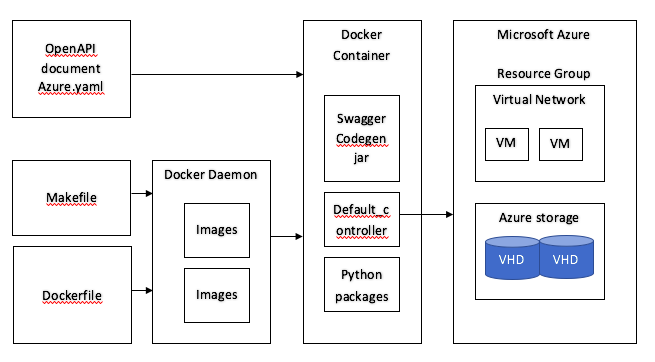
\includegraphics[width=\columnwidth]
        {image/project-architecture.PNG}
        \caption{Project Architecture}\label{fig:project-architecture}
\end{figure}

Figure~\ref{fig:project-architecture} shows the high level architecture of the
project. We can execute this project by using command \textbf{sudo make
docker-all}. Makefile is used to run the service. It creates a docker image
using Dockerfile and then runs it. Swagger codegen installed on docker image
and it is used to generate REST API code for azure swagger specification file.
After that Makefile installs all the python module requirements for the service
. Once the setup is complete Makefile runs the service. Curl call with API path
is used to test the services.



Following technologies have been used in this project:
\begin{itemize}
\item Python 2.7
\item Microsoft azure
\item Swagger Codegen 2.0
\item Docker
\end{itemize}

\section{Background on Technologies Used}
Important technologies used to develop and deploy this project have been
explained below:

\subsection{Microsoft Azure}
Microsoft azure is widely used cloud platform. It provides infrastructure as a
service and platform as a service. It is managed by 19 data centers all over
the world. Azure can be used to host web applications, to store large data
sets, to create virtual machines to for computing purposes and many
more~\cite{hid-sp18-502-microsoft-azure}. It also provides advances
functionality like data analytics and machine learning.
Figure~\ref{fig:azure-architecture} shows architecture for running a linux
virtual machine on Azure. It shows different resources that can be deployed
along with virtual machine like networking and storage components.

 \begin{figure}[!ht]
        \centering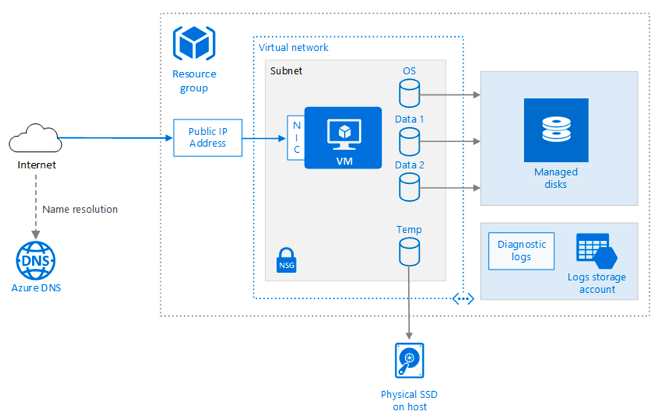
\includegraphics[width=\columnwidth]
        {image/azure-architecture.PNG}
        \caption{Azure Architecture~\cite{hid-sp18-502-azure-archi}}
        \label{fig:azure-architecture}
\end{figure}

Azure uses resource group as logical containers that store different set of
resources together. Virtual machine can be created in the resource group using
existing images published for linux OS~\cite{hid-sp18-502-azure-archi}. By
default on creation of virtual machine OS disk is created for it. OS disk is
part of persistent data that means that it is reliable. One or more data disks
can be created on Azure storage which will be persistent as well. And these
newly created disks can be attached to the virtual machine instant. Azure also
allocates a temporary disk on host machine but it is not persistent against
power outages~\cite{hid-sp18-502-azure-archi}. To communicate
with the virtual machine it should be deployed into a virtual network or a
segment of virtual network called sub network. Also network interface card
should be created for virtual machine to communicate with
network~\cite{hid-sp18-502-azure-archi}. Azure provides distinction between
stopped and de-allocated virtual machines. Azure charges for stopped but does
not charge for de-allocated virtual machines. Also, deleting a virtual machine
does not deletes the VHDs present on azure storage. This helps to keep the data
secure even if the virtual machine gets
deleted~\cite{hid-sp18-502-azure-archi}.


\subsection{Swagger Codegen}
Swagger codegen supports 28 different programming languages. Swagger codegen is
used along with OpenAPI document. OpenAPI has defined set of standards to
create specification for REST API~\cite{hid-sp18-502-swagger}. Swagger codegen
can read OpenAPI document
and generate code in desired programming language with documentation. OpenAPI
is a yaml document in JSON format. It contains swagger version to be used to
develop code along with general description of the REST service which is used
for documentation purpose. It also specifies the type of objects produced and
consumed by REST services. Main components of openAPI file are object
definitions and set of operations~\cite{hid-sp18-502-swagger}. JSON objects
that are used as input or
output of your rest service operations needs to defined in OpenAPI file so that
swagger codegen can read this file and create respective model files to be
used in code.
These object definitions describes all the properties of objects their types.
We can also specify whether the property is required or not. Operations are
defined under paths object~\cite{hid-sp18-502-swagger}. It contains possible
URL endpoints and its
corresponding operation to be invoked. Along with paths, we can specify if
operation requires any input, its type, its location in request. We can also
define set of responses for a given operation~\cite{hid-sp18-502-swagger}.
All these information is used by
swagger codegen to create documentation and proper operation definitions in
controller file. Figure~\ref{fig:swagger-generator} shows how swagger codegen
generates documentation and programs.

\begin{figure}[!ht]
        \centering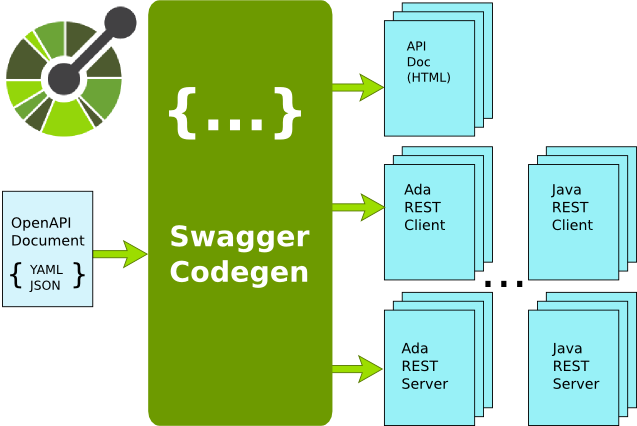
\includegraphics[width=\columnwidth]
        {image/swagger-generator.PNG}
        \caption{Swagger Generator~\cite{hid-sp18-502-swagger}}
        \label{fig:swagger-generator}
\end{figure}

Java is pre-requirement to generate code using swagger. Swagger codegen creates
both server and client side code swagger-codegen jar is executed with -l
parameter to specify the language. For our project we have used python flask
language. We are using swagger version 2.0. We have used the python scripts
generated by swagger codegen to develop REST API.


\subsection{Docker}
Docker is a platform used for running application. It helps programmer to
isolate the infrastructure and actual application. It also helps to develop and
test the application fast to make it ready for
production~\cite{hid-sp18-502-docker}. It allows the
application to run in containers. Containers are similar to virtual machines
but they do not require hypervisor as they run in host machine kernel. This
makes containers light weight. Docker is developed as a client-server
architecture~\cite{hid-sp18-502-docker}. Docker client request docker daemon to
build and run the
containers. Figure~\ref{f:docker} describes the architecture of
docker.

\begin{figure}[!ht]
  \centering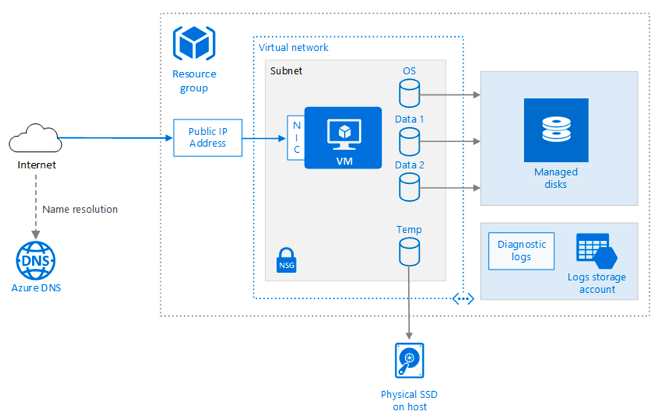
\includegraphics[width=\columnwidth]{image/docker-architecture.PNG}
  \caption{Docker Architecture~\cite{hid-sp18-502-docker}}\label{f:docker}
\end{figure}

Docker client is used by users to send command to docker daemon. Docker
registry is used to store all the docker images\cite{hid-sp18-502-docker}.
Docker registry is public by
default. Images are puller from docker registry using docker pull command.
Docker image can be considered as a blue print or set of instructions that is
used to build a container\cite{hid-sp18-502-docker}. Docker containers are
instance of docker image. Docker services are used to scale the application to
multiple container working
together in the swarm\cite{hid-sp18-502-docker}. In this project docker is used
to create container with ubuntu image and run REST service on it.

\section{Methodology}
This project focuses on identifying objects related to azure for deploying an
instance of a virtual machine on azure using REST API instead of selecting
multiple options via user interface. This can be considered as a part of NIST
Big Data Reference Architecture (NBDRA). Project methodology can be divided in
to documenting various NIST Big Data Reference Architecture Azure resources,
developing REST API to provide interfaces to access or create or
delete individual resources and last part is to configure azure connection
using Azure python APIs.

\subsection{NIST Big Data Reference Architecture (NBDRA)}
NIST Big Data Reference Architecture contains high level components like
security, processing, data, messaging, deployment. These components have
multiple sub-components under them~\cite{hid-sp18-502-nist-vol8}.
Interfaces are needed in order to have
communication between these components. NBDRA focuses on developing interfaces
for that can be used create, manage and monitor resources on Azure, Openstack,
AWS and other such platforms. In this project, I have developed interfaces to
access azure resources~\cite{hid-sp18-502-nist-vol8}. NIST NBDRA volume 8
states few of the Azure objects. As
part of my project, I propose to include following objects to the
documentation. Each object is explained in details below along with its use and
parameters
needed.

\begin{itemize}

\item Azure User Credentials: Azure requires valid subscription in order to
connect to it. Along with subscription id, we require client Id, secret key and
tenant id to be able to create clients to interact with azure platform.

\item Resource Group: Resource groups are created for different types of
resources like virtual machine, networks, databases. Resource groups allows to
partition all the resources of the subscription in sets. This helps to monitor,
access control and manage billing to different resources owned my different
applications of the same company.

\item Virtual Machines: Azure virtual machines are used to create flexible
instance of computer that can be used for computation purposes. We can
customize the virtual machine by selecting hardware profile, data disks,
os-profile and network profile for it. Instances can be scaled later as the
need of the running application grows. Azure charges for running the virtual
machine on per hour basis.

\item IP Address: In order to communicate with Virtual machine we need an IP
address. We can create public IP address using network client. Parameters
needed for creating IP address are location and IP address allocation method.

\item Virtual Network: Virtual network is another Azure resource offered to
allow communication between virtual machines. We can create multiple virtual
networks within a subscription. Azure isolates each virtual network from others
that might belong to different applications.

\item Sub-network: Virtual network can be segmented in one or more subnets. It
is helpful manage and monitor the networks. Azure allocates a part of address
space to each subnet present in the virtual network. We assign virtual machines
to a subnet.

\item Network Interface Card: Virtual Machine needs network interface card in
order to communicate with the virtual network. Network interface card can be
created by passing the public IP address and subnet created for the virtual
machine. Network interface card is used as a network profile information while
creating a virtual machine. A virtual machine can have more than one network
interface card.

\item Data Disk: Virtual Machines require data disks to store the operating
systems, data and applications running on it. Each virtual machine can have one
or more data disks. Data disks can be created by selecting size of the data
disk needed and data disk creation option.

\end{itemize}

\subsection{Swagger RESTful APIs}
An interface was needed to be developed in order to access the objects defined
above. REST service is developed as part of this project to interact with these
objects using swagger. Base path for all the resources will be
\textit{cloudmesh/azure} and it will be common for all the APIs. I have
implemented APIs to lists, lookup by name, create resources. Extra set of API's
are developed to start or stop an instance of virtual machine on azure. List of
all the API's developed and implemented as part of this project are given
below.

\begin{description}
\item \textbf{/resourcegroups}: Returns list of resource groups present under
the subscription provided to resource management client. No parameters needed.

\item \textbf{/resourcegroup/\{id\}}: Returns details for resource group with
the given name. This API needs id that is name of the resource group as
parameter to be present in the path.

\item \textbf{/resourcegroup/create/\{id\}}: This API can be used to create a
new resource group for virtual machines. Resource group name and location are
the parameters needed for this API. Parameters are consumed as a json object.

\item \textbf{/resourcegroup/delete/\{id\}}: This API can be used to delete a
resource group present in the subscription. Input parameter to this API is the
name of the resource group and should be passed within the path of URL.

\item \textbf{/vms/{id}}: This API is used to fetch the list of all the virtual
machines present in a resource group. It can be used to monitor and manage the
virtual machines. Input to this API is the name of the resource group.

\item \textbf{/vm}: This API returns the details of a virtual machine. Input to
this API is a json object resource group and virtual machine name as required
properties of the object. Details of virtual machine includes its hardware
profile, os-profile,storage profile,network profile, id, name and type. These
details can be used to manage a virtual machine and to make decisions while
updating virtual machine.

\item \textbf{/ip/create}: This API is used create a new public IP address to
be used to create a virtual machine. It needs a json object as an input with
parameters as resource group name, IP address name, data center location. It
returns confirmation on successful execution of this operation.

\item \textbf{/vnet/create}: This API is used to create a new virtual private
network within your resource group. It needs a json object as an input with
parameters as resource group name, virtual network name, data center location
and address prefixes. It returns confirmation message on successful execution
of this operation.

\item \textbf{/subnet/create}: This API is used to create subnet within the
virtual network present in the resource group. Input parameters for this API
are resource group name, name of the virtual network, name of the subnet and
address prefixes. Address prefixes for subnet should be a part of address
prefixes given for the virtual network. These parameters are passed using json
object in put method. It returns confirmation message on successful execution
of this operation.

\item \textbf{/nic/create}: One we have created IP adress, virtual network and
subnet for virtual machine, this API can be used to create a network interface
card for the virtual machine. Input parameters needed as part of json object
for this API are name of resource group, virtual network, sub network and IP
address. It returns confirmation message on successful execution of this
operation.

\item \textbf{/vm/create}: This API is used to create virtual machine. This
API needs image reference, network interface card, virtual machine size,
username, password and name for virtual machine as input parameters. It returns
confirmation message on successful execution of this operation.

\item \textbf{/vm/start}: This API is used to start an existing instance to
virtual machine. Parameters needed to start a virtual machine are resource
group name and virtual machine name. Those are passed to this API as json
object. It returns confirmation message on successful execution.

\item \textbf{/vm/stop}: This API is used to stop an existing instance to
virtual machine. Parameters needed to start a virtual machine are resource
group name and virtual machine name. Those are passed to this API as json
object. It returns confirmation message on successful execution.

\item \textbf{/datadisk/create}: This API is used to create a virtual data sidk
for virtual machine to store data. It requires resource group name, data disk
name, location and size of the data disk as input parameters. It returns
confirmation message on successful execution of the operation.

\end{description}

\subsection{Configuration and Connection}
Azure provides set API's to connect to azure through a python program.
Requirement for that is to download the azure python module. In order to
connect to azure from python program we need active azure subscription id and
credentials. Credentials consists of client Id, secret key and tenant id.
Credentials needs to be setup through Azure portal. In order to generate a
client id, first we need to register the App through Azure Active directory. On
registration of the App, azure generates application id which is used as client
id for the credentials. After that, create keys to allow application
communicate with azure. This key is used as secret for the credential. Azure
Active Directory property called Directory id is used as tenant id. Once we
generate credentials, it can be used along with subscription id to create
compute client, network client and resource management client to access these
resources. By default registered App does not get any access to azure
resources. We can assign a role to the App using Access control (IAM). In order
to list all the resources and their details Reader role is enough. But Reader
role wont allow the REST service to create or update the resources. So, I have
assigned contributor role to the application.


\section{Project Artifacts}

Figure~\ref{fig:project-artifacts} lists all the project artifacts created
as part of this project. These files are present in the github directory
project-code.

\begin{figure}[htb]
\begin{verbatim}
Makefile
Dockerfile
azure.yaml
cred.yaml
default_controller.py
\end{verbatim}
\caption{Project Artifacts}\label{fig:project-artifacts}
\end{figure}

Each project artifact is responsible for different part of the project. Details
of working of all the files are given below:
\begin{itemize}

\item \textit{Makefile}: Makefile is used to done all the configuration steps
before we start the service. Makefile is divided into multiple targets each for
different purposes. Docker-build target is used to build a docker container
using Dockerfile and docker-start to run the container. Service target is used
to install swagger codegen, generate code using swagger specification azure
.yaml file, copy controller files in to correct directory and download the
requirements for the service. Start target is used to run the
service. Test target is used to fire curl commands with correct parameters to
test the REST service. Stop target is used for stopping the service. Clean
target is used to remove the code generated by swagger on the container.
docker-stop target is used to stop all the containers. Docker-clean is used to
remove all the existing images.

\item \textit{Dockerfile}: Dockerfile is used to build the required docker
image to run the service on. Dockerfile contains all the requirements like
pulling ubuntu instance, installing python, curl, wget, pip and git. We are
also cloning git repository on the container and setting work directory to
project-code folder. It is also used to download swagger codegen file and to
expose port 8080 for REST service. After that we run service target to complete
the setup.

\item \textit{azure.yaml}: This yaml document file is the swagger specification
used to generate REST API. It contains version of swagger, base path for
API, object definitions, all the API paths and respective input and output
parameters.

\item \textit{cred.yaml}: This file is used to store the authentication
information required to connect to azure. It contains subscription id, client
id, tenant id and secret key. More subscriptions or client ids can be added to
this file if created by user to manage all the subscriptions through same
REST service.

\item \textit{default\_controller.py}: This is the file which contains actual
code to perform the operations. Swagger codegen creates this controller with
the skeleton containing method definitions with parameters and a return
statement. We have constructed the body to perform the respective operations.
This controller file reads authentication details from cred.yaml file and
creates connection to azure by creating compute client, resource client and
network client.

\end{itemize}

\section{Results}

Execution of rest api for all the paths:

\begin{itemize}
\item \textit{Get list of Resource groups}: Figure~\ref{fig:resource-list}
shows command is used to fetch list of resource groups and results.

\begin{figure*}[!ht]
        \centering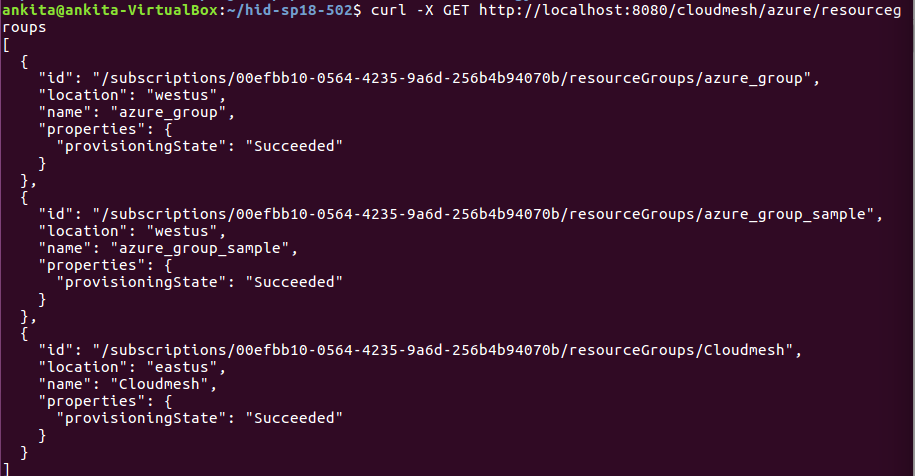
\includegraphics[width=\columnwidth]
        {image/resource-list.PNG}
        \caption{Resource Group List}\label{fig:resource-list}
\end{figure*}

\item \textit{Get list of Virtual Machines}: Figure~\ref{fig:vm-list} shows
command is used to fetch all the virtual machines present under and results.

\begin{figure*}[!ht]
        \centering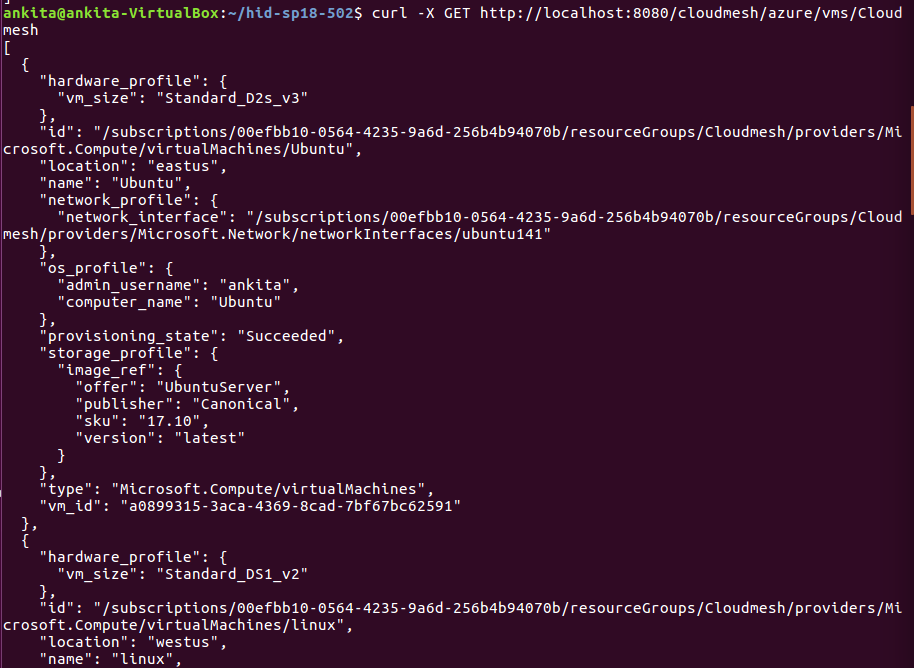
\includegraphics[width=\columnwidth]
        {image/vm-list.PNG}
        \caption{Virtual Machine List}\label{fig:vm-list}
\end{figure*}

\item \textit{Get Resource group by name}: Figure~\ref{fig:get-resource} shows
command is used to get a resource id by name and results.

\begin{figure*}[!ht]
        \centering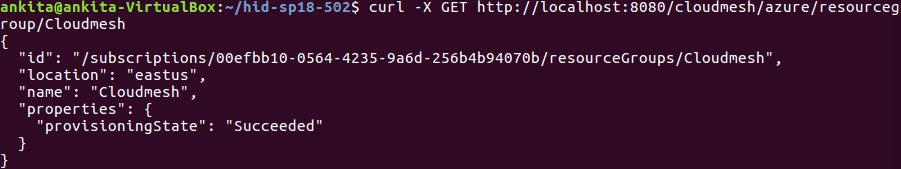
\includegraphics[width=\columnwidth]
        {image/get-resource.PNG}
        \caption{Resource Group by Name}\label{fig:get-resource}
\end{figure*}

\item \textit{Get Virtual Machine by name}: Figure~\ref{fig:get-vm} shows
command is used to get virtual machine by name and results.

\begin{figure*}[!ht]
        \centering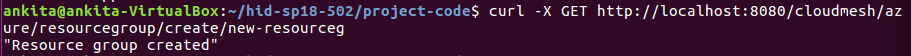
\includegraphics[width=\columnwidth]
        {image/get-vm.PNG}
        \caption{Virtual Machine by Name}\label{fig:get-vm}
\end{figure*}

\item \textit{Create new Resource Group}: Figure~\ref{fig:resource-create}
shows command is used to create new resource group by name and results.

\begin{figure*}[!ht]
        \centering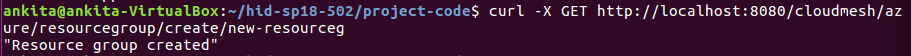
\includegraphics[width=\columnwidth]
        {image/resource-create.PNG}
        \caption{Create Resource Group by Name}\label{fig:resource-create}
\end{figure*}

\item \textit{Create new public IP Address}: Figure~\ref{fig:ip-create} shows
command is used to create public IP address in given resource group and
results.

\begin{figure*}[!ht]
        \centering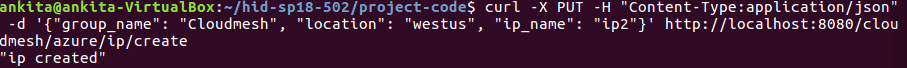
\includegraphics[width=\columnwidth]
        {image/ip-create.PNG}
        \caption{Create IP Address by Name}\label{fig:ip-create}
\end{figure*}

\item \textit{Create new Virtual network}: Figure~\ref{fig:vnet-create} shows
command is used to create new virtual network within given resource group and
results.

\begin{figure*}[!ht]
        \centering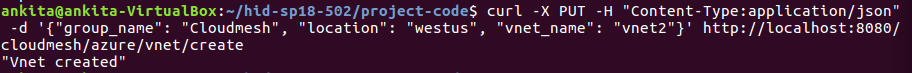
\includegraphics[width=\columnwidth]
        {image/vnet-create.PNG}
        \caption{Create Virtual Network by Name}\label{fig:vnet-create}
\end{figure*}

\item \textit{Create new Virtual sub-network}: Figure~\ref{fig:subnet-create}
shows command is used to create new virtual sub-network within given virtual
network and results.

\begin{figure*}[!ht]
        \centering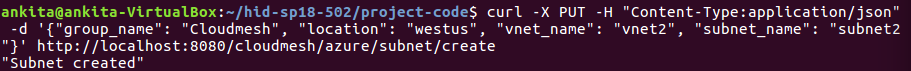
\includegraphics[width=\columnwidth]
        {image/subnet-create.PNG}
        \caption{Create Virtual Sub Network by Name}\label{fig:subnet-create}
\end{figure*}

\item \textit{Create new Network Interface Card}: Figure~\ref{fig:nic-create}
shows command is used create new network interface card and results.

\begin{figure*}[!ht]
        \centering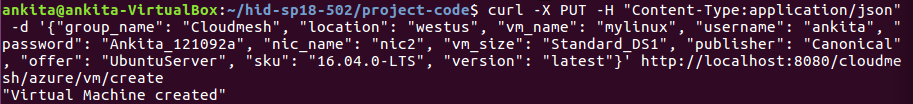
\includegraphics[width=\columnwidth]
        {image/nic-create.PNG}
        \caption{Create Network Interface Card by Name}\label{fig:nic-create}
\end{figure*}

\item \textit{Create new Virtual machine}: Figure~\ref{fig:vm-create} shows
command is used to create virtual machine using vm\_size and image reference
and results. Figure~\ref{fig:azure-vm-created} shows new virtual machine
created on Azure portal.

\begin{figure*}[!ht]
        \centering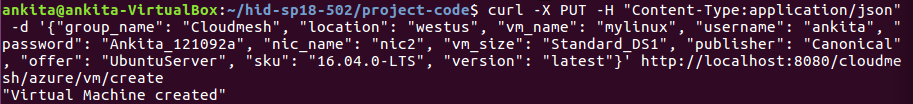
\includegraphics[width=\columnwidth]
        {image/vm-create.PNG}
        \caption{Create Virtual Machine by Name}\label{fig:vm-create}
\end{figure*}

\begin{figure*}[!ht]
        \centering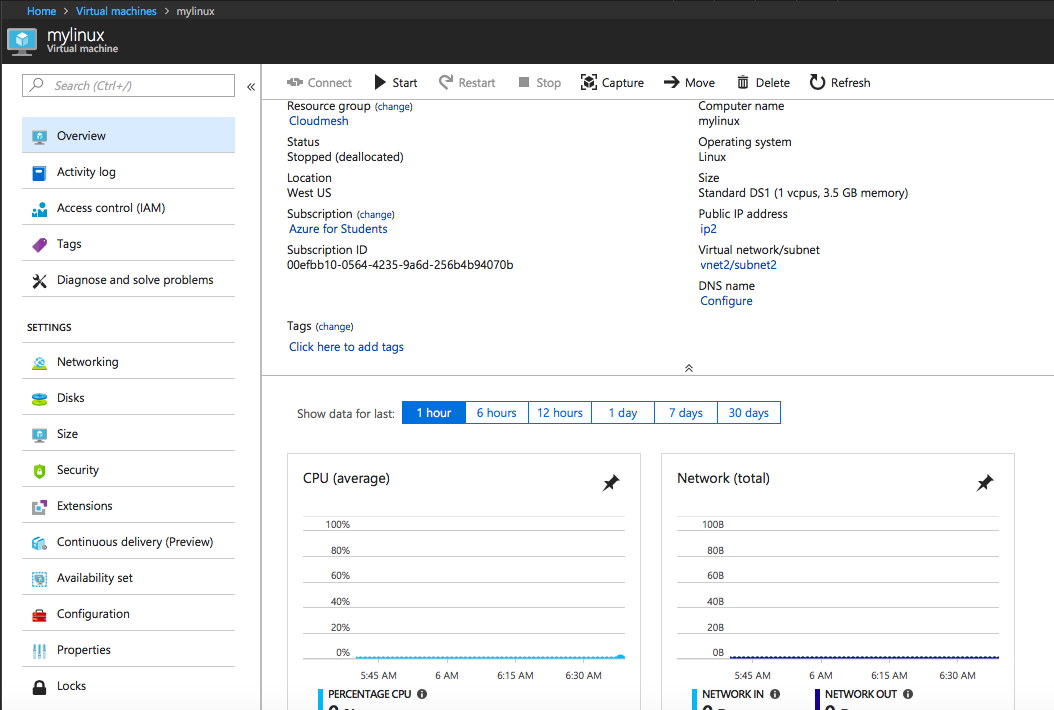
\includegraphics[width=\columnwidth]
        {image/azure-vm-created.PNG}
        \caption{Created Virtual Machine on Portal}\label{fig:azure-vm-created}
\end{figure*}

\item \textit{Start Virtual Machine}: Figure~\ref{fig:vm-start} shows command
is used to start instance of a virtual machine and results.
Figure~\ref{fig:azure-vm-running} shows Ubuntu virtual machine running on Azure
portal.

\begin{figure*}[!ht]
        \centering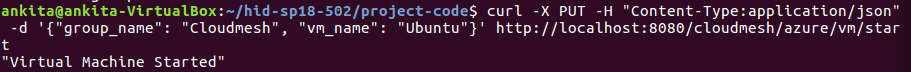
\includegraphics[width=\columnwidth]
        {image/vm-start.PNG}
        \caption{Start Virtual Machine}\label{fig:vm-start}
\end{figure*}

\begin{figure*}[!ht]
        \centering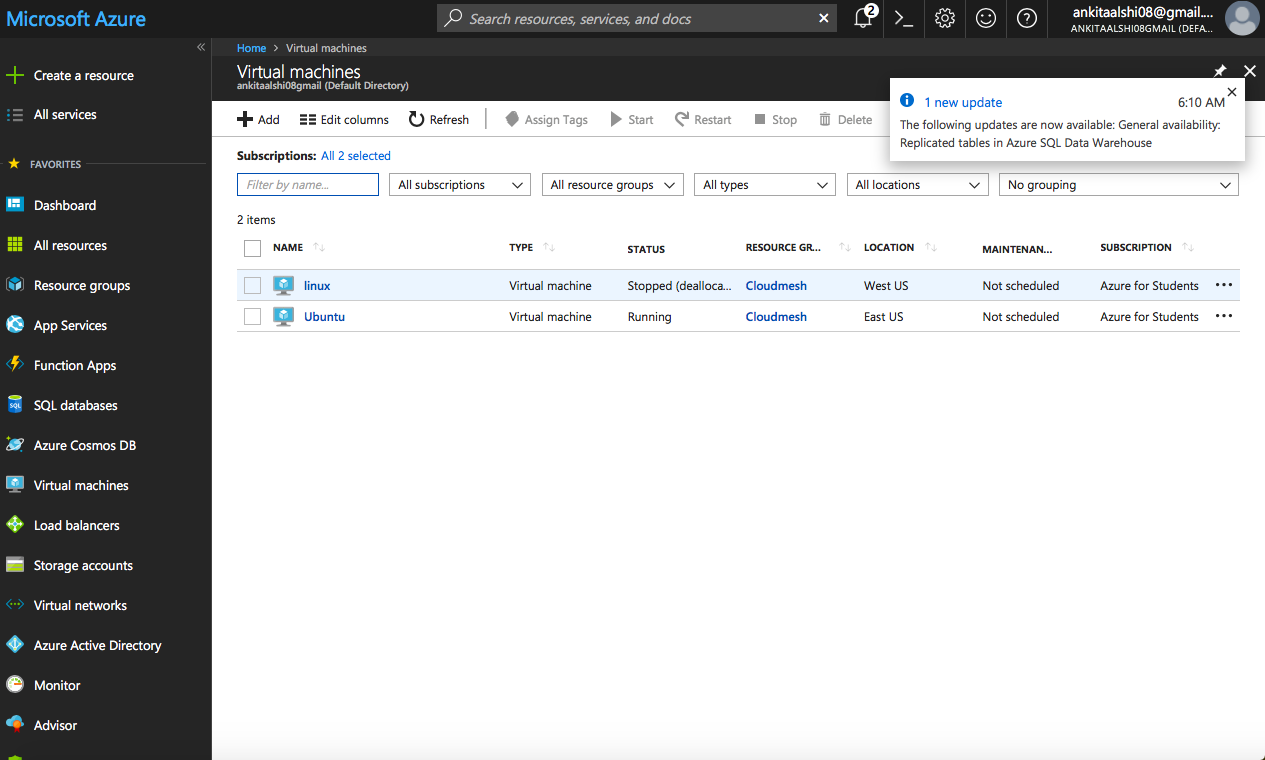
\includegraphics[width=\columnwidth]
        {image/azure-vm-running.PNG}
        \caption{Running Virtual Machine on Portal}\label{fig:azure-vm-running}
\end{figure*}

\item \textit{Stop Virtual Machine}: Figure~\ref{fig:vm-stop} shows command
is used to stop instance of a virtual machine and results.
Figure~\ref{fig:azure-vm-stopped} shows Ubuntu virtual machine stopped on Azure
portal.

\begin{figure*}[!ht]
        \centering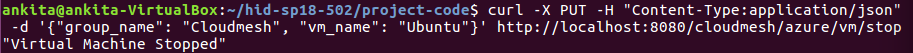
\includegraphics[width=\columnwidth]
        {image/vm-stop.PNG}
        \caption{Stop Virtual Machine}\label{fig:vm-stop}
\end{figure*}

\begin{figure*}[!ht]
        \centering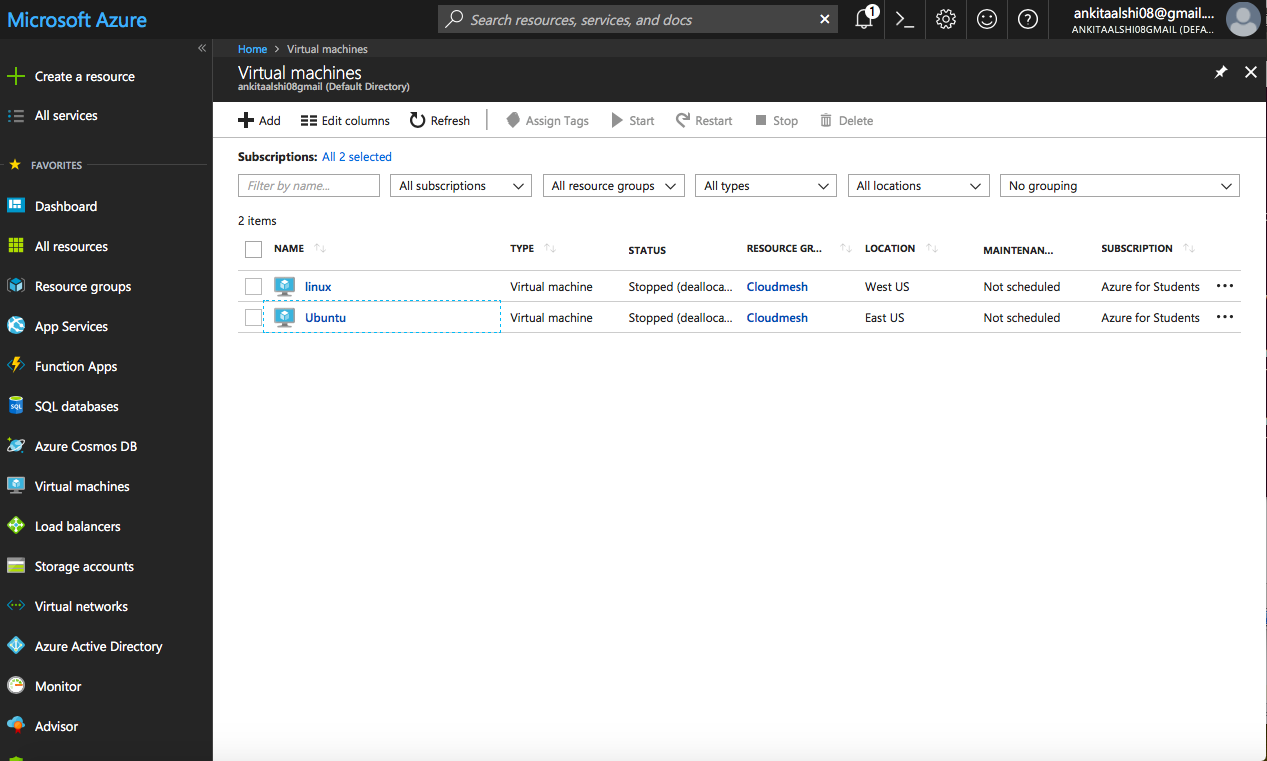
\includegraphics[width=\columnwidth]
        {image/azure-vm-stopped.PNG}
        \caption{Stopped Virtual Machine on Portal}\label{fig:azure-vm-stopped}
\end{figure*}

\end{itemize}

\section{Conclusion}
In this project, we are able to demonstrate how virtual machine instances can
be accessed, created and deployed on Azure platform. We have identified Azure
resource objects with their properties and developed REST service for each one
of them. This project also shows how to use Azure python APIs to get, create
and update resources present under a subscription. We also achieved learning
how to connect to the azure platform and set up required access control to the
application to perform all necessary operations. Project shows how we can
leverage on swagger codegen to create python controllers and models for given
openAPI file. Also major documentation of the operations is also done through
swagger codegen. We also developed ability of run this service on docker
containers by installing azure module on it. This project was focused on only
compute nodes. Future working this project can be to develop APIs to access
storage client, or ability to host an application on the virtual machine
instance.


\begin{acks}

  The author would like to thank Dr.~Gregor~von~Laszewski for his
  support and suggestions to write this paper.

\end{acks}


\bibliographystyle{ACM-Reference-Format}
\bibliography{report} 

